\section{Методы сжатия с потерями}

Лучшие степени сжатия, при сохранении «достаточно хорошего» качества данных. Применяются в основном для сжатия аналоговых данных — звука, изображений. В таких случаях распакованный файл может очень сильно отличаться от оригинала на уровне сравнения «бит в бит», но практически неотличим для человеческого уха или глаза в большинстве практических применений.

\subsection{Дискретно-косинусное преобразование}

Дискретно-косинусное  преобразование представляет  изображение  в  виде  суммы синусоид  с  различной  амплитудой  и  частотой. Одна  из  особенностей  дискретного преобразования Фурье состоит в том, что некоторые локальные участки изображения можно охарактеризовать  небольшим  количеством  коэффициентов  дискретного  преобразования Фурье. Это свойство очень часто используется при разработке методов сжатия изображений. Например,  дискретно-косинусное  преобразование  является  основой  международного стандарта,  который  используется  в  алгоритме  сжатия  изображений  с  потерями  JPEG. Название  формата  <<JPEG>>  состоит  из  первых  букв  названия  рабочей  группы,  которая принимала участие в разработке этого стандарта (Joint Photographic Experts Group)

Двумерное дискретно-косинусное преобразование матрицы A с размерами MxN реализуется согласно следующему выражению:

\[
B_{pq} = \alpha_p \cdot \alpha_q \cdot \sum_{m=0}^{M-1} \sum_{n=0}^{N-1} A_{mn} cos \frac{\pi(2m+1)p}{2M} cos \frac{\pi(2n+1)q}{2N},
\]

где $0 \leq p \leq M-1$ и $0 \leq q \leq N-1$;

\[
    \alpha_p = 
    \begin{cases}
        \frac{1}{\sqrt{M}}, & \text{если } p =0 \\
        \sqrt{\frac{2}{M}}, & \text{если } 1 \leq p \leq M-1
    \end{cases},
    \alpha_q = 
    \begin{cases}
        \frac{1}{\sqrt{N}}, & \text{если } q =0 \\
        \sqrt{\frac{2}{N}}, & \text{если } 1 \leq q \leq N-1
    \end{cases}
\]

Значения $B_{pq}$ называют коэффициентами дискретного косинусного преобразования матрицы $A$.

Обратное дискретное косинусное преобразование реализуется согласно выражениям:

\[
    A_{mn} = \sum_{p=0}^{M-1} \sum_{q=0}^{N-1} \alpha_p \alpha_q B_{pq} cos \frac{\pi(2m+1)p}{2M} cos \frac{\pi(2n+1)q}{2N},
\]

где $0 \leq m \leq M-1$ и $0 \leq n \leq N-1$;

\[
    \alpha_p = 
    \begin{cases}
        \frac{1}{\sqrt{M}}, & \text{если } p =0 \\
        \sqrt{\frac{2}{M}}, & \text{если } 1 \leq p \leq M-1
    \end{cases},
    \alpha_q = 
    \begin{cases}
        \frac{1}{\sqrt{N}}, & \text{если } q =0 \\
        \sqrt{\frac{2}{N}}, & \text{если } 1 \leq q \leq N-1
    \end{cases}
\]

Выражение обратного дискретного косинусного преобразования может интерпретироваться как представление матрицы $A$ с размерами $N \times M$  в виде суммы следующих функций:

\[
    \alpha_p \alpha_q cos \frac{\pi (2m+1)p}{2M} cos \frac{\pi (2n+1)q}{2N}, \text{где } 0 \leq p \leq M-1, 0 \leq q \leq N-1
\]

Эти функции называются основными (базовыми) функциями дискретного косинусного преобразования. Коэффициенты дискретного косинусного преобразования $B_{pq}$ можно рассматривать как весовые при каждой базовой функции. Например, для матрицы с размером  элементов существует 64 базовые функции, что продемонстрировано на рисунке ниже.

\begin{figure}[H]
    \centering
    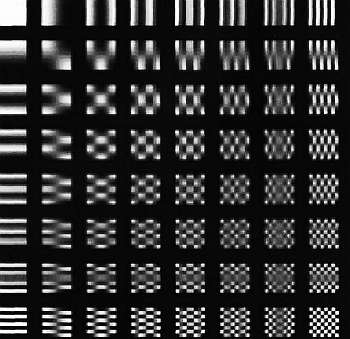
\includegraphics[width=.9\textwidth]{img/dcp-1.jpg}    
    \caption{базовые функции для матрицы 8x8 элементов}
\end{figure}


Горизонтальные частоты увеличиваются слева направо, а вертикальные – сверху вниз.

